\newpage
\section{Introduction}
\label{sec:introduction}
% state the learning objective 

In this laboratory assignment we study a circuit (Fig. 1) containing various elements, to be more specific, 1 capacitor, 7 resistances, 1 independent voltage source $V_s$, 1 dependent voltage source and 1 dependent current source. %In order to study this circuit we use various methods, such as the nodal method, we change the circuit so we can find various variables associated with it, like the $R_{eq}$ and the total solution of $V_6$ and also study the frequency response on the main circuit.%\\

\begin{figure}[H] 

\centering
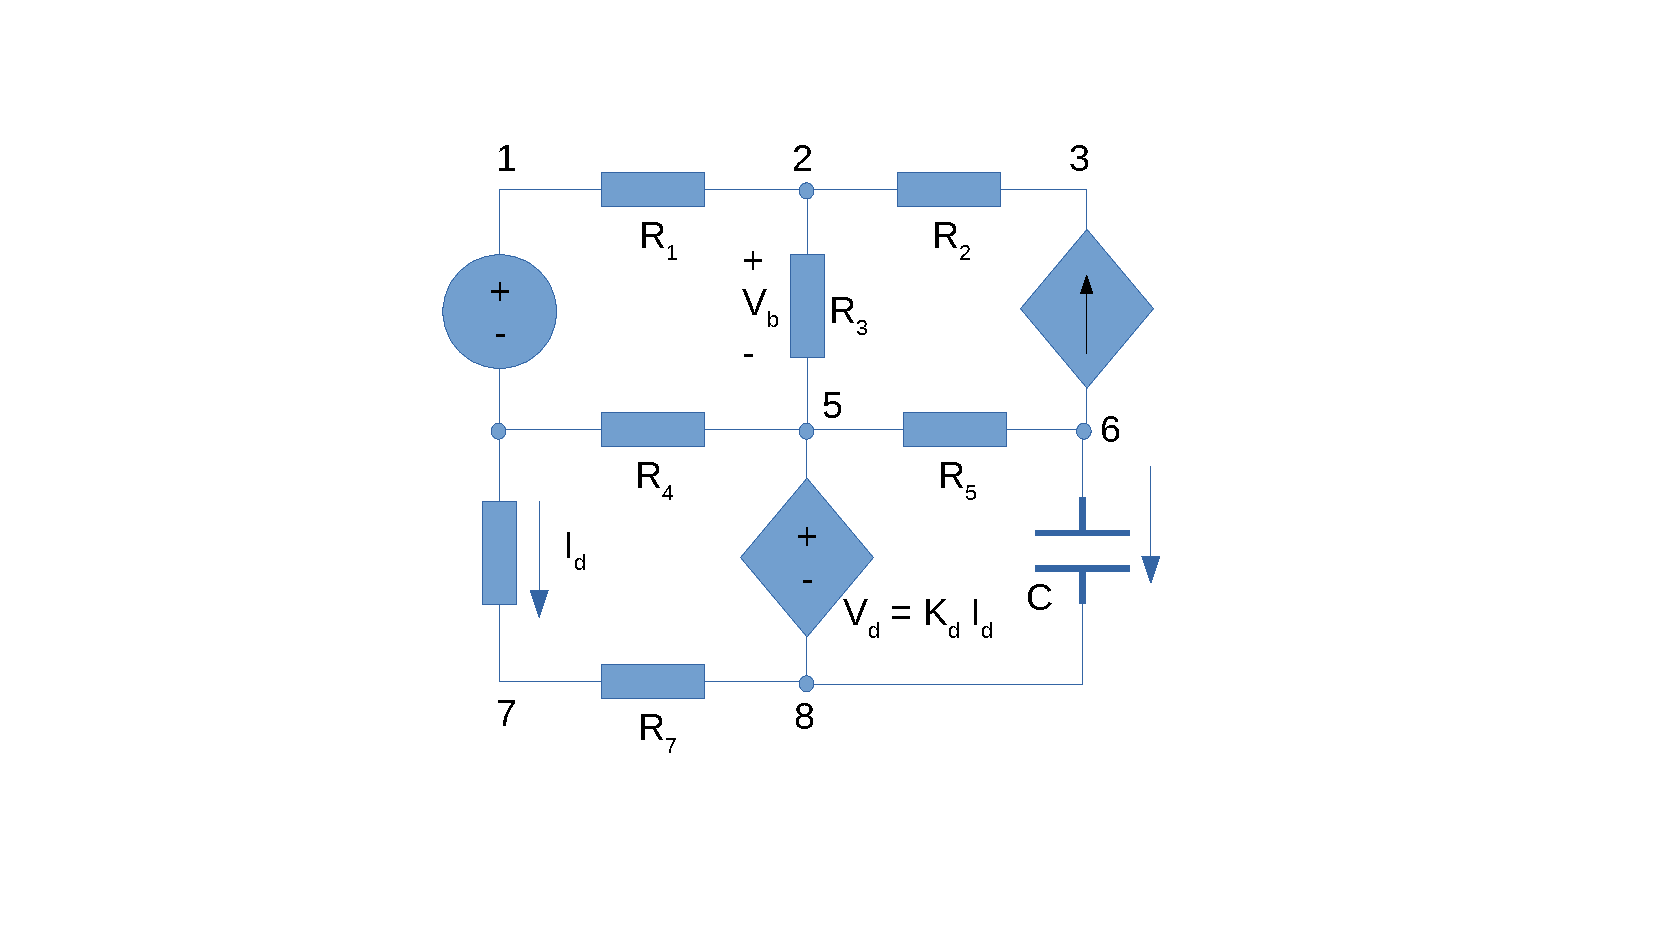
\includegraphics[width=\textwidth]{circuit1.pdf}
\caption{The RC Circuit}
\label{fig:first}

\end{figure}



The independent voltage source $V_s$ varies in time exactly as it follows:

\begin{equation}
V_{s}(t) = V_{s}u(-t) + sin(2 \pi f t)u(t)
\label{equation1}
\end{equation}
Where
\begin{equation}
 u(t)= e
    \begin{cases}
     0 & \text{t $<$ 0}\\
      1 & \text{t $\geq$ 0}
    \end{cases} 
\label{eq:tt}      
\end{equation}


The next table displays the data generated automatically by the Python Script:

\begin{table}[H] \centering
\begin{tabular}{|
>{\columncolor[HTML]{FFCC67}}l |c|}
\hline
\multicolumn{2}{|l|}{\cellcolor[HTML]{EABD8B}Octave - Voltages (V)} \\ \hline
R1 & 1.013609e+03 Ohm\\ \hline
R2 & 2.016578e+03 Ohm\\ \hline
R3 & 3.006816e+03 Ohm\\ \hline
R4 & 4.049229e+03 Ohm\\ \hline
R5 & 3.053925e+03 Ohm\\ \hline
R6 & 2.092502e+03 Ohm\\ \hline
R7 & 1.022320e+03 Ohm\\ \hline
C & 1.029587e-06 F\\ \hline
Kb & 7.213324e-03 A/V \\ \hline
Kd & 8.321035e+03 V/A \\ \hline

\end{tabular}
\caption{Initial data}
\end{table}


In Section~\ref{sec:analysis}, a theoretical analysis of the circuit is
presented. In Section~\ref{sec:simulation}, the circuit is analysed by
simulation, and the results are compared to the theoretical results obtained in
Section~\ref{sec:analysis}. The conclusions of this study are outlined in
Section~\ref{sec:conclusion}. \\


